% \cleardoublepage
% ==============================================================
\chapter{Proteomatic workflow for proteogenomic genome annotation}
\label{appendix-b}
% \markboth{Appendix B: Proteomatic workflow for proteogenomic genome annotation}{Appendix B: Proteomatic workflow for proteogenomic genome annotation}
% \addcontentsline{toc}{chapter}{Appendix B: Proteomatic workflow for proteogenomic genome annotation}
% ==============================================================

% ==============================================================
% \renewcommand{\baselinestretch}{1.0} 
% \renewcommand{\arraystretch}{1.0} 
% ==============================================================

% \begin{figure}
% \clearpage
\vfill
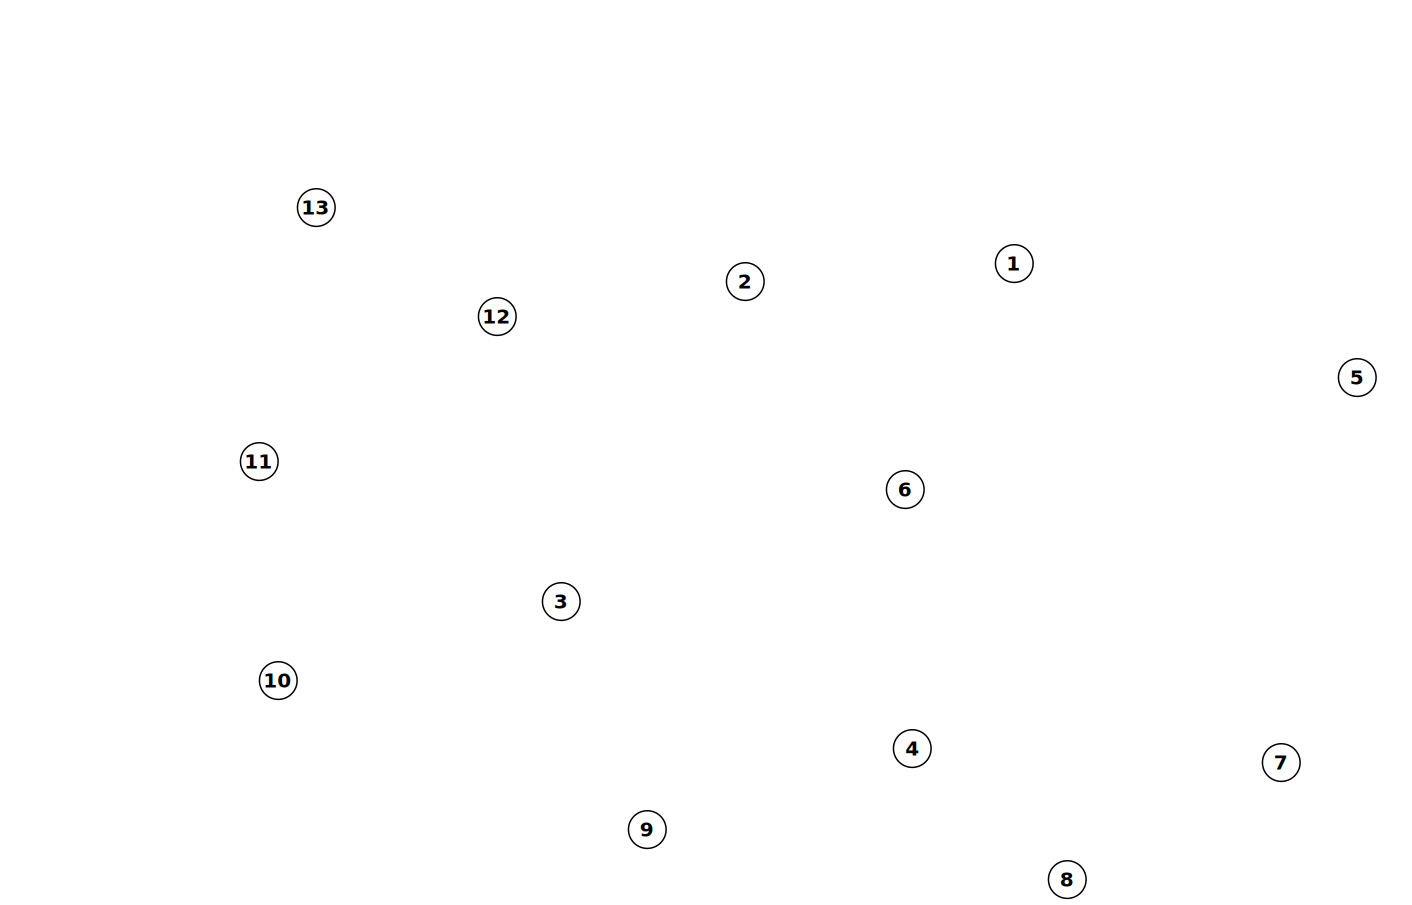
\includegraphics[width=\textwidth]{figures/gpf-annotation-2.jpg}
% \caption{
%     {\bf Proteomatic pipeline for the generation of GPF peptide hints
%     for proteogenomic genome annotation via AUGUSTUS.}
%     Apart from the {\em de novo} sequencing step, performed using
%     PEAKS, all remaining tools in the pipeline are freely available
%     and automatically downloaded by Proteomatic.
% }
% \label{fig:appendix-b-pipeline}
% \end{figure}
\vfill
\clearpage



The depicted workflow is composed of the following processing steps:

\begin{enumerate}

\item {\bf {\em De novo} sequencing.} 
PEAKS is used to determine 10 candidates peptides for each MS/MS spectrum
via {\em de novo} sequencing.

\item {\bf GPF alignment.} 
The {\em de novo} sequences peptides are aligned to the genomic DNA sequence 
of \cre, allowing for a maximum intron length of 602 base pairs and considering 
a single splice site motif of GT/AG. 
This process reduces the size of the candidate peptide set per MS/MS spectrum 
from 10 to 3.4 on average.
The output contains detailed information of where each peptide alignment
is located in the genomic DNA sequence.

\item {\bf Extract peptides.}
All resulting peptides are extracted from the GPF result tables for each 
SDS-PAGE band.

\item {\bf Create FASTA databases.}
For each band, a FASTA database is created which contains all GPF peptides 
obtained from that band.

\item {\bf Create a target/decoy database.} 
A previous version of the gene models is used to create a target/decoy database.
While the gene models used are potentially incomplete, we assume that most
of the contained sequences are correct, thus qualifying the database to be
used as a provider of target peptides.

\item {\bf Run OMSSA.} 
The database search program OMSSA is run once for each input file using
the gene model target/decoy database and all GPF peptides obtained from
the respective band.

\item {\bf Sanitize peptide/spectral matches.} 
A {\em hit distinctiveness filter} is applied to the lists of peptide/spectral
matches (PSM) resulting from OMSSA, yielding a single result file that contains
the results from all bands.
The filter employed checks whether there are multiple peptide assignments
to the same MS/MS scan and discards non-first-ranking PSM.
In addition, all PSM to a MS/MS scan are discarded if the top-scoring PSM
is not distinctive enough because a different peptide was assigned with a 
comparably good score.

\item {\bf Filter by FDR.} 
An E-value threshold is determined for the entire PSM list.
For the FDR estimation, only the PSM to the target/decoy database generated
from the gene models are regarded, but the final E-value threshold is applied
to all PSM, including the matches to GPF peptides.

\item {\bf Filter by mass accuracy.} 
In order to compensate for the fact that the OMSSA version used in the pipeline
only allows to specify mass accuracies in Da, the resulting PSM list is
filtered again to discard all matches with a relative mass error of more
than 5 ppm.

\item {\bf Dicard gene model peptides.} 
Every PSM in the result list originates from either the gene models or the
GPF peptide set. If a peptide occurs in both sources, it is listed twice in
the PSM list.
At this stage, this information is used to discard all hits to gene models,
resulting in a list of statistically significant, gene model-independent 
peptides deduced via PEAKS and GPF.

\item {\bf Extract GPF peptides.} 
Because the various details provided by OMSSA are no longer required,
all resulting peptides are extracted from the PSM list.

\item {\bf Merge GPF alignment information.} 
The GPF results for each band are combined into a single file because the
final processing step 13 requires a single input file with genomic alignment
information for peptides.

\item {\bf Generate AUGUSTUS hints.} 
Finally, the list of confidently identified peptides and the table containing
all information about where these peptides are located within the genome
is combined to create the final GFF file which can directly be used by AUGUSTUS.
In this processing step, non-spliced alignments are preferred over spliced 
alignments.
Furthermore, all peptides for which multiple alignments exist are discarded.

\end{enumerate}

